\chapter{Tao Concepts}
\label{c:concepts}

\tao stands for ``Tool for Accelerator Optics''. \tao is a general
purpose program for simulating high energy particle beams in
accelerators and storage rings. This tutorial assumes you are already
familiar with the basics of particle beam dynamics and its
formalism. There are several books that introduce the topics very
well. A good place to start is \textit{The Physics of Particle
Accelerators} by Klaus Wille.

\index{Bmad}
\tao is based on the \bmad\cite{b:bmad} subroutine library. An
understanding of the nitty-gritty details of the routines that
comprise \bmad is not necessary, however, one should be familiar with
the conventions that \bmad uses and this is covered in the \bmad
manual.

So, what is \tao good for? A large variety of applications. It's
versatility is that it's easily expandable. Think of it as an
accelerator design and analysis environment. But even without any
customizations, \tao will do much analysis. 

This chapter discusses how \tao is organized. After you are familiar
with the basics of \tao, there is a hands-on tutorial in
Chapter~\sref{c:tutorial}. After you get more familiar with \tao, you
might be interested exploit its versatility by extending \tao to do
custom calculations. For this, see Chapter~\ref{c:custom.tao}.

%----------------------------------------------------------------
\section{The Organization of Tao: The Super\_Universe}
\label{s:organization}

Many simulation problems fall into one of three categories: 
\begin{itemize}
\item 
Design a lattice subject to various constraints.
\item
Simulate errors and changes in machine parameters. For example, you want to
simulate what happens to the orbit, beta function, etc., when you change
something in the machine. 
\item 
Simulate machine commissioning including simulating data measurement and
correction. For example, you want to know what steering strength changes will
make an orbit flat.
\end{itemize}
Programs that are written to solve these types of problems have common
elements: You have variables you want to vary in your model of your
machine, you have "data" that you want to view, and, in the first two
categories above, you want to match the machine model to the data (in
designing a lattice the constraints correspond to the data).

With this in mind, \tao was structured to implement the essential
ingredients needed to solve these simulation problems.  
The information that \tao knows about can be divided into five
(overlapping) categories:
\begin{description}
  \index{Lattice}
  \item[Lattice] \Newline   
Machine layout and component strengths, and the beam orbit (\sref{s:lattice}).
  \index{Data}
  \item[Data] \Newline
Anything that can be measured.
For example: The orbit of a particle or the lattice beta 
functions, etc. (\sref{c:data})
  \index{Varialbe}
  \item[Variables] \Newline
Essentially, any lattice parameter or initial condition that can be varied.
For example: quadrupole strengths, etc. (\sref{s:variable.overview}).
  \index{Plotting}
  \item[Plotting]  \Newline
Information used to draw graphs, display the lattice 
floor plan, etc. (\sref{s:plotting}).
  \index{Global parameters}
  \item[Global Parameters] \Newline
 \tao has a set of parameters to control every aspect of how it behavies from
the random number seed \tao uses to what optimizer is used for fitting data.
\end{description}

%------------------------------------------------------------------------
\section{The Super\_universe}
\label{s:super.uni}
\index{Super_universe}
\index{Structure}
The information in \tao deals is organized in a hierarchy of
\vn{``structures''}. At the top level, everything known to \tao is
placed in a single structure called the \vn{super_universe}.

Within the \vn{super_universe}, lies one or more \vn{universes}
(\sref{s:universe}), each \vn{universe} containing a particular
machine lattice and its associated data. This allows for the user to
do analysis on multiple machines or multiple configurations of a
single machine at the same time. The \vn{super_universe} also contains
the \vn{variable}, \vn{plotting}, and \vn{global parameter} information.

%------------------------------------------------------------------------
\section{The Universe}
\label{s:universe}
\index{Universe!textbf}

\index{Lattice}\index{Design lattice}\index{Model lattice}\index{Base lattice}
\index{Data}
The \tao \vn{super_universe} (\sref{s:super.uni}) contains one or
more \vn{universes}.  A \vn{universe} contains a \vn{lattice}
(\sref{s:lattice}) plus whatever data (\sref{c:data}) one wishes to
study within this lattice (i.e. twiss parameters, orbit, phase,
etc.). Actually, there are three lattices within each universe: the
\textbf{design} lattice, \textbf{model} lattice and \textbf{base}
lattice. Initially, when \tao is started, all three lattices are
identical and correspond to the lattice read in from the lattice
description file (\sref{s:init.lat}).

There are several situations in which multiple universes are
useful. One case is where there are multiple machines. For example, a
transfer line connected to a storage ring. In this case, one universe
will correspond to the transfer line and another universe will
correspond to the storage ring. 

Another case where multiple universes are useful is where data has
been taken under different machine conditions. For example, suppose
that a set of beam orbits have been measured in a storage ring with
each orbit corresponding to a different steering element being set to some
non-zero value. To determine what
quadrupole settings will best reproduce the data, multiple universes can be
setup, one universe for each of the orbit measurements. Variables can be
defined to simultaneously vary the corresponding quadrupoles in each
universe and \tao's built in optimizer can vary the variables until
the data as determined from the \vn{model} lattice (\sref{s:lattice})
matches the measured data. This \vn{orbit response matrix} (ORM) analysis
is, in fact, a widly used procedure at many laboratories.

%------------------------------------------------------------------------
\section{Lattices}
\index{Lattice!textbf}
\label{s:lattice}

A \vn{lattice} consists of a machine description (the strength and
placement of elements such as quadrupoles and bends, etc.), along with the
beam orbit through them. There are actually three types of lattices:
  \vspace*{-3ex}
  \begin{description}
  \index{Design lattice!textbf}
  \item[Design Lattice] \Newline 
The \vn{design} lattice corresponds to the lattice read in from the
lattice description file(s) (\sref{s:init.lat}). In many instances, this
is the particular lattice that one wants the actual physical machine
to conform to. The \vn{design} lattice is fixed. Nothing is allowed to
vary in this lattice.
  \index{Model lattice!textbf}
  \item[Model Lattice] \Newline
Except for some commands that explicitly set the \vn{base} lattice,
all \tao commands to vary lattice variables vary quantities in the
\vn{model} lattice. In particular, things like orbit correction
involve varying \vn{model} lattice variables until the \vn{data},
as calculated from the \vn{model}, matches the \vn{data} as actually measured.
  \index{Base lattice!textbf}
  \index{Base lattice!using set command}
  \item[Base Lattice] \Newline
It is sometimes convenient to designate a reference lattice so that
changes in the \vn{model} from the reference point can be examined.
This reference lattice is called the \vn{base} lattice. The \vn{set}
command (\sref{s:set}) is used to transfer information from the
\vn{design} or \vn{model} lattices to the base lattice.
  \end{description}

%------------------------------------------------------------------------
\section{Variables}
\label{s:variable.overview}
\index{Variables}

\index{Change command}
\index{Optimizer!variables}
A variable is anything that can be varied. For example, quadrupole
strengths or the initial position of a particle in a LINAC. Any
variable can be varied using the \vn{change} command
(\sref{s:change}). However it can be convenient to set up within \tao
predefined groups of variables. For example, the optimizer
(\sref{s:optimizer}) will only work with such blocks.

Variables control attributes of elements in the model lattice of one
or more universes. They are not the same thing as attributes in
lattice elements.  Instead, they \textit{control} attributes in
lattice elements. They are more akin to \bmad \textit{overlays}. A
given variable may control a single attribute of one element in one or
more universes. If you want a variable to control a collection of
elements like a \bmad \textit{group} then you need to insert the
appropriate group element in your lattice. Variables are what you vary in
order to change your model lattice. You can also change your model
lattice by directly changing and lattice element attribute. However,
if you plan on doing any optimization then you will need to use
variables.

\index{Variables!v1_var}
Blocks of variables are associated with what is called a \vn{v1_var}
structure and each of these structures has a \vn{name} with which to
refer to them in \tao commands. For example, if \vn{quad_k1} is the
name of a \vn{v1_var}, then \vn{quad_k1[5]} referres to the variable 
with index 5 in the block. 

A set of variables within a \vn{v1_var} block
can be referred to by using using a comma \vn{,} to
separate their indexes. Additionally, a colan \vn{:} can be use to
specify a range of variables. For example
\begin{example}
  quad_k1[3:6,23]
\end{example}
refers to variables 3, 4, 5, 6, and 23. Instead of a number, the
associated lattice element name can be used so if, in the above
example, the lattice element named \vn{q01} is assocaited with
\vn{quad_k1[1]}, etc., then the following is equivalent:
\begin{example}
  quad_k1[q03:q06,q23]
\end{example}
Using lattice names instead of numbers is not valid if the same
lattice element is associated with more than one variable in a
\vn{v1_var} array. This can happen, for example, if one variable controls
an element's \vn{x_offset} and another variable controlls the same element's
\vn{y_offset}. 

A given variable may control a single attribute of one element in a
\vn{model} lattice of a single universe or it can be configured to
simultaneously control an element attribute across multiple
universes. Any one variable cannot control more than one attribute of
one element. However, a variable may control an overlay or group
element which, in turn, can control numerous elements.

Each individual variable has a number of values associated with it:
  \vspace*{-3ex}
  \index{Variable!measured}\index{Variable!reference}
  \index{Variable!model}\index{Variable!design}\index{Variable!base}
  \begin{description}
  \item[Measured Value] \Newline
The Value as obtained at the time of the \vn{data} measurement.
  \item[Reference Value] \Newline
The Value as obtained at the time of the \vn{reference} data  measurement.
  \item[Model Value] \Newline
The value as given in the \vn{model} lattice.
  \item[Design Value] \Newline
The value as given in the \vn{design} lattice.
  \item[Base Value] \Newline
The value as given in the \vn{base} lattice.
  \end{description}
These components and others can be refered to using the notaion
\vn{|name} where \vn{name} is the appropriate name for the
component. The list of components that can be set or refered to are:
\begin{example}
  quad_k1[1]|meas      ! Value at time of data measurement
  quad_k1[1]|ref       ! VAlue at time of the reference data measurement
  quad_k1[1]|model     ! Value in the model lattice
  quad_k1[1]|base      ! Value in the base lattice
  quad_k1[1]|design    ! Value in  the design lattice
  quad_k1[1]|weight    ! Weight used in the merit function.
  quad_k1[1]|old       ! Scratch value.
  quad_k1[1]|step      ! For fitting/optimization: What is considered a small change.
  quad_k1[1]|exists    ! Logical
  quad_k1[1]|good_var  ! Logical
  quad_k1[1]|good_ref  ! Logical
  quad_k1[1]|good_user ! Logical
  quad_k1[1]|good_opt  ! Logical
  quad_k1[1]|good_plot ! Logical
\end{example}

Use the \vn{show var} (\sref{s:show}) command to view variable information

%------------------------------------------------------------------------
\section{Plotting}\index{Plotting}
\label{s:plotting}

\begin{figure}[tb]
  \centering
  \includegraphics{plot.eps}
  \caption[A plot has a collection of graphs.]
{A plot has a collection of graphs and a graph has a 
collection of curves. A plot becomes visible when it is associated
with some region on the page using the \vn{place} command. Note that
on the actual page the plot/region border is not visible.}
  \label{f:plot}
\end{figure}

Some definitions:
  \vspace*{-3ex}
\begin{description}
\index{Curve|textbf}
\item[Curve] \Newline
A \vn{curve} is a set of (x,y) points to be plotted.
\index{Graph|textbf}
\item[Graph] \Newline
A \vn{graph} consists of horizontal and vertical axes along with a set
of \vn{curve}s that are plotted within the graph. 
\index{Plot|textbf}
\item[Plot] \Newline
A \vn{plot} is essentially a collection of \vn{graphs}.
\index{Page|textbf}
\item[Page] \Newline
The \vn{page} refers to the Xwindow where graphics are displayed or the 
corresponding printed graphics page.
\index{Region}
\item[Region] \Newline
The \vn{page} is divided up into a number of rectangles called
\vn{regions}. \vn{Regions} may overlap.
\end{description}

\index{Template plot}\index{Region}\index{Place command}
\index{Graph}\index{Plot!initialization file}\index{Curve}
The plot initialization file (cf.~Chapter~\ref{c:init}) defines a set
of \vn{template plots}. A \vn{template} defines what type of data is
to be plotted (orbit, beta function, etc.), how many \vn{graphs} there are,
what the scales are for the \vn{graph} axes, how the \vn{graph}s are
laid out, etc.  The plot initialization file also defines a set of
\vn{region}s within the \vn{page}. Any \vn{template plot} can be
placed in any region. Using the \vn{place} command (see
Chapter~\ref{c:command} for a full descriptions of all commands) one
can assign a particular \vn{template plot} to a particular region for
plotting.  The relationship between \vn{region}, \vn{plot},
\vn{graph}, and \vn{curve} is shown graphically in
Figure~\ref{f:plot}.

Figures~\ref{f:plot.page1} and \ref{f:plot.page2} show examples of a
plot \vn{page}. Figure~\ref{f:plot.page1} was generated by defining
two regions called \vn{top} and \vn{bottom} in the plot initialization
file. The \vn{top} region was defined to cover the upper half of the
\vn{page} and the \vn{bottom} region was defined to cover the bottom
half. \vn{Template plots} were defined to plot phase and orbit data
from a defined set of detector elements in the lattice. Each
\vn{template plot} defined two graphs which in both cases where
assigned the names \vn{x} and \vn{y}. The orbit \vn{template plot} was
placed in the \vn{top} region and the phase \vn{template plot} was
placed in the \vn{bottom} region. The horizontal axis numbering is by
detector \vn{index}.  Displayed plots are referred to by the
\vn{region} name (\vn{top} and \vn{bottom} in this case). Individual
graphs and curves are referred to using the nomenclature
\vn{region.graph.curve}. Thus, in this example, the horizontal orbit graph
would be referred to as \vn{top.x}.  Using the \vn{plot} command one
can then specify \vn{who} is plotted. \vn{who} refers to
\vn{measured}, \vn{reference}, \vn{model}, \vn{base}, and/or
\vn{design} data.  Notice that the same \vn{template plot} can be
assigned to different \vn{regions} and the plots in different
\vn{regions} can have different scales for their axes or different
\vn{who}. In the example in Figure~\ref{f:plot.page1}, \vn{who} for
the \vn{top} plot is \vn{model} and for the \vn{bottom} plot it is
\vn{model - design}.

Plots may be referred to by their template name or by the name of the
region they are placed in. For example, the orbit plot in
Figure~\ref{f:plot.page1} may be referred to using the region name
(\vn{top}) or the template name (\vn{orbit}). A template may be placed
in multiple regions.  For example, you may wish to plot the \vn{model}
data for the orbit in one region and the \vn{design} data for the
orbit in another region. In this case the command \vn{scale orbit}
would scale the plots in both regions while to scale the plot in only
one of the regions you would need to use the region name. A graph of a
plot is specified using the format \vn{plot_name.graph_name} where
\vn{plot_name} is a template or region name and \vn{graph_name} is the
name of the graph. For example, if the horizontal orbit graph of the
]\vn{orbit} plot is named \vn{x} then it would be referred to as
\vn{orbit.x} or \vn{top.x}. A curve within a graph is specified using
the format \vn{plot_name.graph_name.curve_name}.

The \vn{use}, \vn{veto}, \vn{restore}, and \vn{clip} commands are used
to control what data is used in fitting the model to the data in the
optimization process (see Chapter~\ref{c:opti}). The general rule is
that these commands only effect measured and reference data. If
plotting \vn{model}, \vn{design} and/or \vn{base} data then the data
will be displayed irregardless. If plotting \vn{meas} and/or \vn{ref} data
then the data displayed will vary with these commands.  \vn{meas} or
\vn{ref} data vetoed for display is also vetoed for fitting.  However,
measured data that is off the vetical or horizontal scale may still be
used by the optimizer unless vetoed with the \vn{veto} or \vn{clip}
command.  If there are data points off the vertical scale then
``**Limited**'' will appear in the upper right-hand corner of the
graph. If plotting measured data then these points off scale will
still be used by the optimizer.

The \vn{x-axis} and \vn{x-scale} commands are used to set the axis
type and scale for each graph. The axis type can be either \vn{index},
\vn{ele_index} or \vn{s} which corresponds to the data index number,
element index number and longitudinal poisition in the lattice (from
element 0) respectively.

Figure~\ref{f:plot.page2} shows another example of a plot \vn{page}.
In this case the \vn{page} was generated by again defining two
vertically stacked regions but in this case the regions have different
heights.  A \vn{template plot} with a single graph was placed in the
bottommost \vn{region}.  This \vn{graph} contains a \vn{key_table}.
A \vn{key_table} is used in conjunction with \vn{single mode} and is
explained in Chapter~\ref{c:single}. A \vn{template plot} containing
five \vn{graphs} was placed in the uppermost region. The uppermost
\vn{graph} of this \vn{template plot} contains a \vn{lat_layout} which
shows the placement of lattice elements.  What elements are displayed
in a \vn{lat_layout} and what shapes they are represented by is
specified in the initialization file. The horizontal scale is
longitudinal position (\vn{s}).  The remaining four graphs show
dispersion and beta data from two different universes representing the
low energy and high energy transport in an energy recovery linac. The
individual data points here (hard to see in this example) have been
slaved to the \vn{lat_layout} and represent the beta and dispersion at
the edges of the displayed elements in the \vn{lat_layout}.


\begin{figure}
  \centering
  \includegraphics[width=5in]{plot-page1.eps}
  \caption{Example of a plot page}
  \label{f:plot.page1}
\end{figure}

\begin{figure}
  \centering
  \includegraphics[width=5in]{plot-page2.eps}
  \caption{Another example of a plot page.}
  \label{f:plot.page2}
\end{figure}

\vfill
\break
%------------------------------------------------------------------------
\section{Single Character Input}
\index{Single Mode}

Sometimes it is convenient to be able to vary variables using single
key strokes without having to type a carriage return.  With \tao, this
is possible using what is called \vn{single mode}. This is distinct
from \vn{line mode} where commands to \tao are typed at the command
line with a carriage return signaling the end of the command. 

The \vn{single mode} initialization file associates variables with
certain keyboard keys so that when these keys are pressed the value of
the variable is varied. This association between variables and keys is
called a \vn{key table}. See Chapter~\sref{c:single} for more details.

%------------------------------------------------------------------------
\section{Tracking Types}
\index{Tracking!Types}

\index{track_type}
\index{tao_global_struct}
\index{Global%track_type}
The are two types of tracking implemented in \tao: single particle
tracking and many particle multi-bunch tracking.
Single particle tracking is just that, the
tracking of a single particle through the lattice. Many particle
multi-bunch tracking creates a gaussian distribution of particles at
the beginning of the lattice and tracks each particle through the
lattice, including any wakefields. 
Single particle tracking is used by default. The
\vn{global%track_type} parameter (\sref{s:globals}), which is set in
the initialization file, is used to set the tracking.

Particle spin tracking has also been set up for single particle and many
particle tracking. See Sections~\sref{s:globals} and \sref{s:beam.init} for
details on setting up spin tracking.

%------------------------------------------------------------------------
\section{Lattice Calculation}\index{Lattice!calculation of}
\label{s:lat.calc}

After each \tao command is processed, the lattice and ``merit''
function are recalculated and the plot window is regenerated. The
merit function determines how well the \vn{model} fits the measured
data. See Chapter~\ref{c:opti} for more information on the merit
function and its use by the optimizer.

Below are the steps taken after each \tao command execution:
\begin{enumerate}
  \item 
The data and variables used by the optimizer is re-determined. This is
affected by commands such as \vn{use, veto,} and \vn{restore} and any
changes in the status of elements in the ring (e.g. if any elements
have been turned off).
  \item 
If changes have been made to the lattice (e.g. variables changed) then
the model lattice for all universes will be recalculated. The
\vn{model} orbit, linear transfer matrices and twiss parameters are
recalculated for every element. All data types will also be calculated
at each element specified in the initialiation file.  For single
particle tracking the linear transfer matrices and twiss parameters
are found about the tracked orbit. Tracking is
performed using the tracking method defined for each element
(i.e. Bmad Standard, Symplectic Lie, etc...). See the \bmad Reference
manual for details on tracking and finding the linear transfer
matrices and twiss parameters.
  \item 
The \vn{model} data is recalculated from the \vn{model} orbit, linear
transfer matrices, twiss parameters, particle beam information and
global lattice parameters.  Any custom data type calculations are
performed \textit{before} the standard \tao data types are calculated.
  \item 
Any user specified data post-processing is performed in
\vn{tao_hook_post_process_data}.
  \item 
The contributions to the merit function from the variables and data are
computed.
  \item 
Data and variable values are transfered to the plotting structures.
  \item 
The plotting window is regenerated.
\end{enumerate}

